\documentclass{standalone}
\usepackage{tikz}
\usepackage{amsmath}

\begin{document}

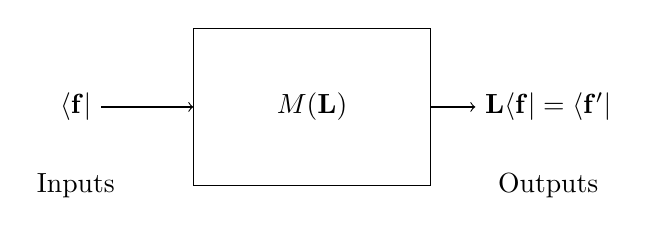
\begin{tikzpicture}
    % Node styles
    \tikzstyle{block} = [draw, rectangle, minimum height=2cm, minimum width=3cm]
    
    % Nodes
    \node at (0, 0) (inputs) {$\langle {\bf f} \rvert$};
    \node [block, right of=inputs, node distance=3cm] (system) {$M({\bf L})$};
    \node [right of=system, node distance=3cm] (outputs) {${\bf L}\langle {\bf f} \rvert = \langle {\bf f'} \rvert$};
    
    % Labels
    \node [below of=inputs, node distance=1cm] {Inputs};
    \node [below of=outputs, node distance=1cm] {Outputs};
    
    % Arrows
    \draw [->] (inputs) -- (system);
    \draw [->] (system) -- (outputs);
\end{tikzpicture}

\end{document}